\begin{proof}
    Начав с произвольной вершины, пройдём по рёбрам графа, не проходя ни по какому ребру дважды. Мы не сможем сделать следующий шаг только в двух случаях: либо мы вернёмся в вершину, где уже были (это будет означать, что в графе есть цикл), либо вернёмся в вершину степени 1.

    Определим две операции:
    \begin{enumerate}
        \item Если в графе есть вершина степени 1, то удалим её вместе с ребром, которому она принадлежит.
        \item Если в графе есть цикл, то удалим любое ребро из этого цикла, не удаляя вершин, которым принадлежит это ребро.
    \end{enumerate}

    Мы можем выполнять эти операции, пока у графа есть рёбра. Значит, процесс остановится только тогда, когда граф состоит из одной вершины и не имеет рёбер (а для этого графа соотношение \eqref{eyler} выполнено).

    Осталось понять, что при выполнении вышеуказанных операций число $B - P + \Gamma$ не меняется.

    Первая операция: \[B \to B - 1\] \[P \to P - 1\]
    Вторая операция: \[B \to B\] \[P \to P - 1\]
    
    Отметим, что при выполнении обеих операций число $\Gamma$ не увеличивается (очевидно, что если некоторые точки можно было соединить непрерывной кривой, не пересекая рёбра графа, то после удаления ребра их можно будет соединить той же кривой).

    Осталось доказать, что для операции 1 число компонент не меняется, а для операции 2 число компонент уменьшается ровно на 1. Доказательство проводится примерно так же, как и доказательство теоремы Жордана для ломаных (см. шаг 1, где мы описывали процесс хождения вдоль рёбер замкнутой ломаной).

    Для операции 1: надо проверить, что если для точек $P,Q \notin G$ существует непрерывная кривая $\gamma$, соединяющая $P$ с $Q$ и не пересекающая рёбра, отличные от $e$ (т.е. ребро, которое мы удаляем), то существует другая непрерывная кривая $\tilde{\gamma}$, соединяющая $P$ с $Q$ и не пересекающая рёбра.

    \begin{figure}[h]
        \centering
        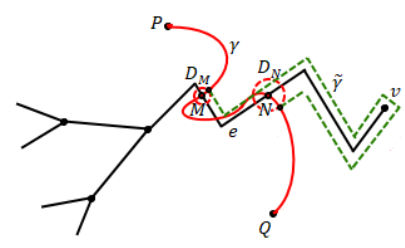
\includegraphics[scale=0.8]{images/c6.1.png}
        \caption{Существование кривой $\tilde{\gamma}$.}
        \label{fig:c6.1}
    \end{figure}

    Рассмотрим $M$ — первую точку на кривой $\gamma$, принадлежащую ребру $e$ и $N$ — последнюю точку на кривой $\gamma$, пересекающую ребро $e$ (они существуют, так как образ ребра $e$ — замкнутое подмножество плоскости).

    Рассмотрим замкнутый круг $D_M$ с центром в точке $M$, не пересекающий другие рёбра и пересекающийся с ребром $e$ по двум радиусам (аналогично для точки $N$ рассмотрим круг $D_N$). Из точки $P$ пройдём по кривой $\gamma$ до первой точки, принадлежащей кругу $D_M$, затем пройдём вдоль ломаной до последней точки на кривой $\gamma$, принадлежащей кругу $D_N$, а из неё по кривой $\gamma$ пройдём до точки $Q$ — получим непрерывную кривую $\gamma$, соединяющую точки $P$ и $Q$, и не пересекающую рёбра, отличные от $e$.

    Для операции 2: поскольку цикл не самопересекающийся, его образ при вложении графа в плоскость можно рассматривать как замкнутую не самопересекающуюся ломаную. По теореме Жордана для ломаных, этот цикл разбивает плоскость на две компоненты.

    Рассмотрим замкнутый круг с центром в точке, лежащей на ребре ломаной. Если точки $A$ и $B$ лежат в разных компонентах, на которые рёбра ломаной разбивают круг, тогда точки $A$ и $B$ лежат в разных компонентах относительно этой замкнутой ломаной (это следует из доказательства теоремы Жордана для ломаных). Тогда тем более точки $A$ и $B$ лежат в разных компонентах относительно графа $G$.

    После удаления ребра $e$ очевидно, что эти точки можно соединить непрерывной кривой (например, отрезком), см.рис.\ref{fig:c6.2}.

    \begin{figure}[h]
        \centering
        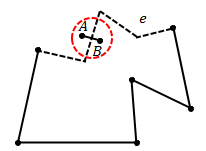
\includegraphics[scale=0.8]{images/c6.2.png}
        \caption{Соединение точек $A$ и $B$, лежащих в разных компонентах.}
        \label{fig:c6.2}
    \end{figure}

    Таким образом, мы доказали, что после операции 2 число компонент уменьшится. Осталось показать, что оно уменьшится ровно на 1.

    Поймём, какие точки, которые были в разных компонентах до удаления ребра, могут оказаться в одной компоненте после удаления ребра. Рассмотрим точки $P$ и $Q$, такие что до удаления ребра их нельзя было соединить непрерывной кривой, не пересекая рёбра графа, а после удаления — можно. Это означает, в частности, что кривая $\gamma$, соединяющая $P$ и $Q$, пересекает только ребро $e$.

    На кривой $\gamma$ рассмотрим первую и последнюю точки ($M$ и $N$, соответственно) пересечения этой кривой с ребром $e$. Рассмотрим замкнутые круги $D_M$ и $D_N$ с центрами в этих точках и докажем, что точки $P$ и $Q$ можно соединить с одной из точек $A$ или $B$ непрерывной кривой, не пересекая рёбер графа.

    \begin{figure}[h]
        \centering
        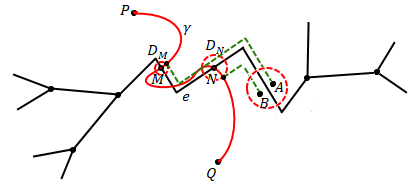
\includegraphics[scale=0.8]{images/c6.3.png}
        \caption{Точки $P$ и $Q$ можно соединить с одной из точек $A$ или $B$.}
        \label{fig:c6.3}
    \end{figure}

    Из точки $P$ пойдём по кривой $\gamma$ до первой точки пересечения с кругом $D_M$, затем пойдём вдоль ребра $e$ и соединим эту точку либо с точкой $A$, либо с точкой $B$, состоит из части кривой $\gamma$ и некоторого пути вдоль ломаной.

    Аналогично для точки $Q$ — пойдём по кривой $\gamma$ до первой точки пересечения с кругом $D_N$, затем пойдём вдоль ребра $e$ до точки $A$ или $B$ (см. рис.\ref{fig:c6.3}).

    Мы доказали, что точка $P$ до удаления ребра $e$ лежит в одной из компонент, которой принадлежат либо точка $A$, либо точка $B$, а точка $Q$ лежит во второй из этих компонент (так как точки $A$ и $B$ находятся в разных компонентах). Это и означает, что при удалении ребра $e$ сливаются (становятся одной компонентой) только те компоненты, которые задаются выбранными нами точками $A$ и $B$. Значит, число компонент уменьшится ровно на 1.

    Таким образом, при указанных операциях число $B - P + \Gamma$ не меняется, и если в конце процесса (для графа, состоящего из одной точки), оно равно 2, то и для начального графа выполняется соотношение
    \[B - P + \Gamma = 2.\]
\end{proof}

\begin{theorem}[Критерий Понтрягина-Куратовского]
    Граф планарен тогда и только тогда, когда он не содержит подграфов, гомеоморфных $K_5$ и $K_{3,3}$.
\end{theorem}
\begin{proof}
    Без доказательства.
\end{proof}

\newpage
\section{Многогранники}
\subsection{Основные определения}
\begin{definition}
    \textit{Многоугольник (на плоскости)} — множество точек, ограниченное замкнутой вложенной конечнозвенной ломаной (вместе с этой ломаной).
\end{definition}

\begin{definition}
    Два многоугольника, расположенных в пространстве, называются \textit{смежными по ребру $a$}, если $a$ — их общее ребро. %и это отношение симметрично (т.е. если $K$ смежен по ребру $a$ с $M$, то и $M$ смежен по ребру $a$ с $K$).
\end{definition}

\begin{definition}
    \textit{Многогранная поверхность} — это конечный набор многоугольников в $\R^3$ такой, что для любого ребра любого многоугольника существует единственный другой многоугольник, смежный с ним по данному ребру (причём это отношение симметрично).
\end{definition}

\begin{definition}
    Многогранная поверхность называется \textit{вложенной}, если выполнены следующие условия:
    \begin{enumerate}
        \item Внутренние точки граней принадлежат только этим граням.
        \item Внутренние точки рёбер принадлежат только тем двум граням, которые смежны по данному ребру.
        \item У любой вершины существует «обход»: все грани, соответствующие данной вершине (как точке в $\R^3$) таковы, что для любых двух граней существует цепочка граней, их соединяющая. Причём все они смежные по рёбрам, инцидентных данной вершине.
        %\item Для любой вершины все грани, которым она принадлежит, образуют замкнутую цепочку граней, смежных по рёбрам, содержащих эту вершину. 
    \end{enumerate}
    То есть, у любой точки существует окрестность, гомеоморфная двумерному диску.
\end{definition}

\begin{definition}
    Многогранная поверхность \textit{связна}, если для любых двух граней существует цепочка граней, смежных по ребрам, их соединяющая.
\end{definition}

\begin{remark}
    Мы будем рассматривать только связные и вложенные многогранные поверхности.
\end{remark}

\begin{definition}
    Пусть дана вложенная связная многогранная поверхность $L$. Компактная часть пространства, ограниченная $L$ вместе с поверхностью $L$, называется \textit{многогранником}.
\end{definition}

\begin{definition}
    Множество в $\R^n$ называется \textit{выпуклым}, если для любых двух точек в нём, оно содержит весь отрезок между ними (отрезок, их соединяющий).
\end{definition}

\begin{definition}[1]
    Многогранник \textit{выпуклый}, если его множество точек выпукло.
\end{definition}

\begin{definition}[2]
    Многогранник \textit{выпуклый}, если он лежит в одном полупространстве, образованном плоскостью, содержащем любую его грань.
\end{definition}

\begin{definition}[3]
    Многогранник \textit{выпуклый}, если он совпадает (как множество в $\R^3$) с выпуклой оболочкой его вершин (выпуклая оболочка множества — это минимальное выпуклое множество, его содержащее).
\end{definition}

\begin{theorem}
    Определения (1)-(3) эквивалентны.
\end{theorem}
\begin{proof}
    $(1) \Longrightarrow (2)$. Рассмотрим некоторую грань многогранника и плоскость $\alpha$, содержащую эту грань. Предположим, что многогранник $M$ не содержится целиком в одном из полупространств, на которые плоскость $\alpha$ разбивает пространство, т.е. существуют две точки $P \in M, \ Q \in M$, расположенные по разные стороны от плоскости $\alpha$.
    \begin{figure}[h]
        \centering
        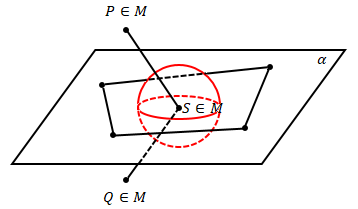
\includegraphics[scale=0.8]{images/c6.4.png}
        \caption{Точки $P \in M, \ Q \in M$, расположенные по разные стороны от плоскости $\alpha$.}
        \label{fig:c6.4}
    \end{figure}
    Рассмотрим $S$ — произвольную внутреннюю точку грани, лежащей в плоскости $\alpha$, и соединим её с точками $P$ и $Q$. Так как многогранник $M$ выпуклый, то отрезки $PS$ и $QS$ также принадлежат $M$.

    Рассмотрим маленький шар с центром в точке $S$. Его пересечение с гранью, в которой лежит точка $S$ — круг, который делит шар на два полушара, причём точки одного полушара не принадлежат $M$, а точки другого полушара принадлежат $M$ (т.к. $S$ — внутренняя точка грани).

    Тем самым получаем противоречие — отрезки $PS$ и $QS$ целиком принадлежат многограннику, но часть одного из этих отрезков неминуемо попадёт в полушарие, точки которого не принадлежат многограннику $M$.

    $(2) \Longrightarrow (1)$. Рассмотрим $W$ — пересечение всех полупространств, о которых идёт речь в определении (2). Многогранник $M$ лежит в этом пересечении, потому что он лежит по одну сторону от каждой грани в каждом из этих полупространств: $M \subset W$.

    $W$ — выпуклое подмножество (как пересечение выпуклых подмножеств пространства). Докажем, что $M = W$, т.е. любая точка пересечения полупространств является точкой многогранника.

    Предположим, что это не так, то есть существуют точки $P \in W, \ Q \in W$ такие, что $P \in M, \ Q \notin M$. Тогда отрезок $PQ$ пересечёт одну из граней многогранника, а значит, пересечёт и плоскость, содержащую эту грань, но мы выбирали точки $P$ и $Q$ так, чтобы они лежали в одном полупространстве для любой плоскости, содержащей одну из граней многогранника — противоречие, значит, $M = W$.

    $(3) \Longrightarrow (1)$. Очевидно, так как выпуклая оболочка множества — это некоторое выпуклое подмножество.

    $(1) \Longrightarrow (3)$. Пусть многогранник $M$ является выпуклым в смысле определения (1). Рассмотрим множество $W$ — выпуклую оболочку его вершин. Очевидно, что $W \subset M$. Докажем, что $M \subset W$, т.е. что все точки многогранника будут принадлежать выпуклой оболочке вершин. У многогранника есть 4 типа точек: вершины, внутренние точки рёбер, внутренние точки граней, внутренние точки многогранника.

    Вершины (по определению) принадлежат выпуклой оболочке вершин. Рассмотрим произвольную внутреннюю точку ребра. Поскольку его концы (как вершины) принадлежат множеству $W$, то и весь отрезок с концами в этих точках тоже принадлежит $W$, поэтому все внутренние точки рёбер также принадлежат $W$.

    Рассмотрим внутреннюю точку грани. Проведём в плоскости, содержащей эту грань, прямую — она пересечёт стороны многоугольника, про которые мы уже знаем (поскольку это вершины или внутренние точки рёбер), что они принадлежат $W$, поэтому и весь отрезок с концами в этих точках также принадлежит $W$. Стало быть, внутренние точки граней также принадлежат $W$.

    Рассмотрим внутреннюю точку многогранника. Проведём через неё прямую, которая пересечёт грани многогранника в точках, про которые мы уже знаем, что они принадлежат $W$. Стало быть, внутренние точки многогранника также принадлежат $W$.
\end{proof}